\chapter{Reliability Analysis}
\chaptermark{Reliability}

We will define reliability analysis to be the analysis of the \emph{time} to \emph{failure}.
We will also assume that ``time'' and ``failure'' are well defined and agreed upon.

We intuitively understand ``more reliable'' to mean ``lasts longer''. 
We should also consider, however, the case of a product that is designed to fail after some time, thus forcing the consumer to buy a new one. 
Some may say that a major hi-tech company named after a fruit employs this practice, which is known as \emph{planned obsolescence}\footnote{\url{https://en.wikipedia.org/wiki/Planned_obsolescence}.}
Be it true or not, I hope we can agree that good knowledge of your product's life expectancy is a desirable. 

By ``product'' we clearly imply a production problem, but our methods equally apply to other problems where we analyse the distribution of times-to-events. 
\begin{description}
	\item[Services] The analysis of time-to-service in service queues. 
	\item[Marketing] The analysis of time-to-adoption/abandon in marketing. 
	\item[Sotware reliability] The analysis of time-to-bug in software reliability.
	\item[Actuary] The analysis of time-to-death in actuary sciences (insurance).
	\item[Pharmaceutics] The analysis of time-to-effect in pharmaceutics. 
	\item[Epidemiology] The analysis of time-to-infection/recovery in epidemiology and biostatistics. 
\end{description}

Reliability analysis involves the study of a probabilistic property of our product- its \emph{survival}.
Any probabilistic model will require calibration to reality via data. 
This chapter thus introduces both the probability calculus typically used for reliability analysis, and then some statistical considerations involved when calibrating these models.



\section{Probabilistic Analysis}




\subsection{A Static View}

Let $\x_j \in \set{0,1}, j=1,\dots,p$ denote the state of the $j$'th component of a system, and $x=(x_1,\dots,x_p)$.

\begin{definition}[Structure Function]
The \emph{structure function}, $\struct=\struct(x):x \mapsto \set{0,1}$, is an indicator function of the state of the system. A failure indicated by $0$. 
\end{definition}

\begin{remark}[$\Phi$]
We apologize to the reader for using $\Phi$ to denote both the $\gauss{0,1}$ CDF, and the structure function.
We do so to stay in accordance with reliability literature, and since no collisions are created in this chapter by doing so.
\end{remark}

\begin{definition}[Series System]
A \emph{series system}, or \emph{serial system}, is one where all components need to function for the system to function: $$\struct(x)=\prod_{j=1}^{p}x_j.$$
\end{definition}
A reliability diagram of a series system is given in Figure~\ref{fig:series_system}.
\begin{figure}[ht]
\centering
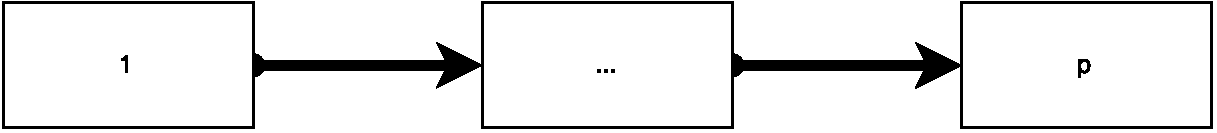
\includegraphics[width=0.5\linewidth]{art/series_system}
\caption{Series system.}
\label{fig:series_system}
\end{figure}


\begin{definition}[Parallel System]
A \emph{parallel system} is one where all components need to fail for the system to fail:
$$\struct(x)=1-\prod_{j=1}^{p} (1-x_j)= \coprod_{j=1}^p x_j.$$
\end{definition}
A reliability diagram of a parallel system is given in Figure~\ref{fig:parallel_system}.
\begin{figure}[ht]
\centering
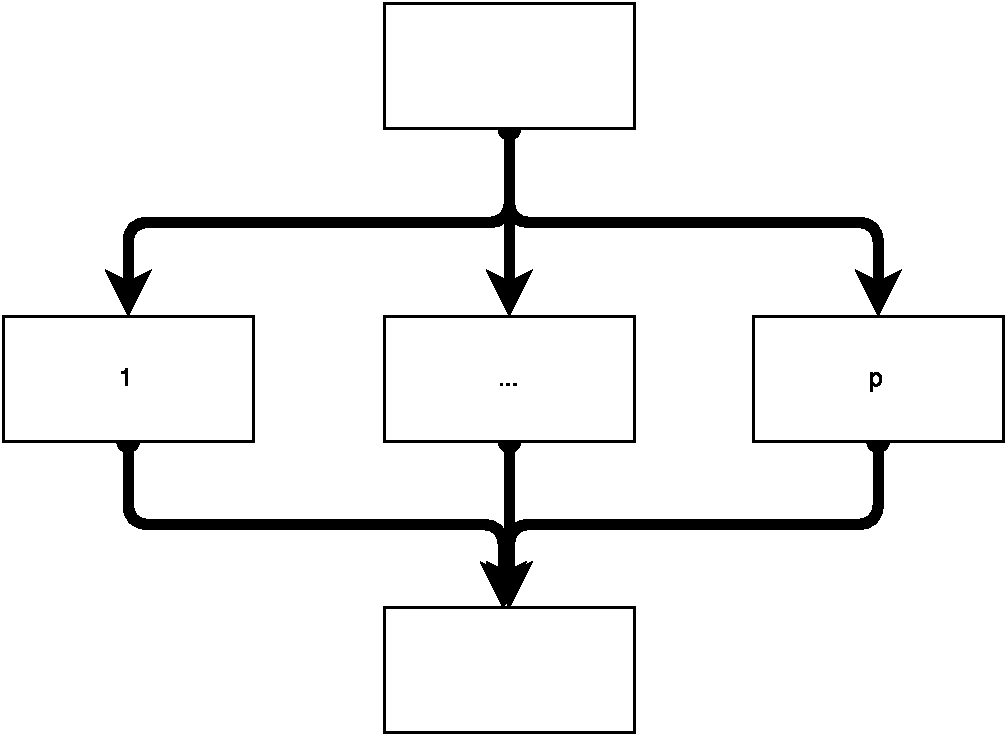
\includegraphics[width=0.5\linewidth]{art/parallel_system}
\caption{Parallel system.}
\label{fig:parallel_system}
\end{figure}





\begin{definition}[k-out-of-p System]
A \emph{k-out-of-p} system is one where at least $k$ components need to function for the system to function:
$$\struct(x)=\indicator{\sum_{j=1}^{p} x_j \geq k}.$$
\end{definition}



\begin{think}
	A reliability diagram of a k-out-of-p system is not provided, since it is not very friendly. Try thinking of a 2-out-of-3 system to see why.
\end{think}



\begin{definition}[Monotone System]
A system is said to be \emph{monotone} if $\struct(x_1,\dots,x_p)$ is non decreasing in all components.
\end{definition}
The definition of monotonicity captures the idea that you cannot improve a system's state by breaking components.
This seems rather natural (I am still looking for a counter example).


\begin{think}
	Think how the structure function of a non monotone system would look.
\end{think}




\begin{definition}[Reliability]
We define the \emph{reliabity of component $j$} to be $$p_j:= P(\x_j=1),$$ 
and  the \emph{reliability of the system} 
$$ S_\struct = S_{\struct(x)}:=P(\struct(x)=1).$$
\end{definition}


\begin{example}[Reliability of a series system]
For $\Phi(x)$ a series system, assuming independent components, we have
$$ S_\struct= \prod_{j=1}^{p} p_j.$$
\end{example}


\begin{example}[Reliability of a parallel system]
For $\Phi(x)$ a parallel system, assuming independent components, we have
$$ S_\struct= 1-\prod_{j=1}^{p} (1-p_j)= \coprod_{j=1}^p p_j. $$
\end{example}


\begin{example}[Reliability of a k-out-of-p system]
For $\Phi(x)$ a k-out-of-p system, assuming independent components with equal reliability ($p_i=p_0$), we have
$$ S_\struct= \sum_{i=k}^{p} \binom{p}{i} p_0^i (1-p_0)^{p-i} .$$
\end{example}



\subsubsection{State enumeration method}
To compute the reliability of more complex structures, the brute-force approach is the \emph{state enumeration method}. 
This method simply relies on summation of the probabilities of the states for which the system functions.
$$ S_\struct= \sum_{x} \Phi(x) P(\x=x).$$


\subsubsection{Factoring method}
The \emph{factoring method}, \aka \emph{pivot-decomposition method}, relies on two ingredients: 
(a) conditioning on the state of some components greatly simplifies the structure, and
(b) the total probability argument.
Combining the two we have:
$$ S_\struct= p_j  S_{\struct|x_j=1} + (1-p_j) S_{\struct|x_j=0}   ,$$
where $S_{\struct|x_j=1}$ denotes the reliability of the structure $\Phi$ conditional on $x_j=1$.
The following example demonstrates the power of the factoring method.

\begin{example}[Bridge Structure]
\label{eg:bridge}
Consider structure in Figure~\ref{fig:bridge}.
To compute the reliability, we will call upon the factoring method while conditioning on the state of component $3$:
$$ S_\struct= p_3  S_{\struct|x_3=1} + (1-p_3) S_{\struct|x_3=0}   .$$
Now note that when $x_3=1$ then we have a series structure of parallel structures, while when $x_3=0$ we have a parallel structure of series structures.:
\begin{align*}
	S_{\struct|x_3=1} &= (p_1 \coprod p_2) (p_4 \coprod p_5),\\
	S_{\struct|x_3=0} &=  p_1 p_4 \coprod p_2 p_5,
\end{align*}
so that 
$$ 	
	S_\struct = p_3  (p_1 \coprod p_2) (p_4 \coprod p_5) + (1-p_3) (p_1 p_4 \coprod p_2 p_5).
$$
\begin{figure}[ht]
\centering
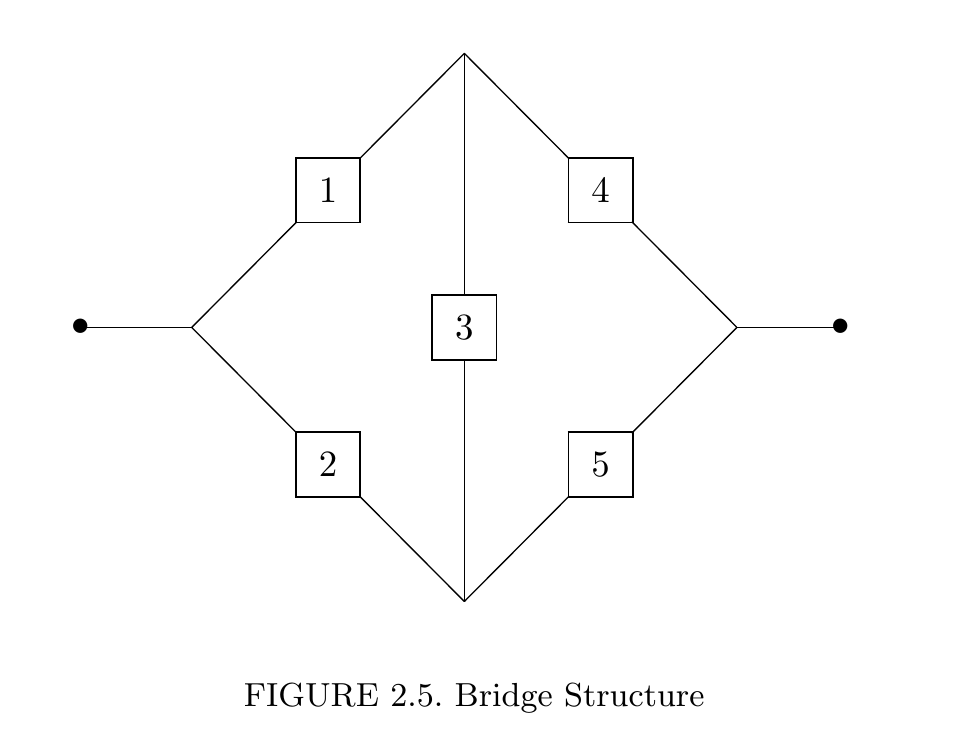
\includegraphics[width=0.5\linewidth]{art/bridge}
\caption[Bridge Structure]{Structure of a bridge system. Source: \cite[Fig.2.5]{aven_stochastic_1999}}
\label{fig:bridge}
\end{figure}
\end{example}
Example~\ref{eg:bridge} demonstrates a single application of the factoring method. Clearly, it can be applied recursively for more complicated systems.

The example also demonstrates a more general principle. Namely, that redundancy is preferable at the component level, and not at the system's level.
Put differently- when designing a backup, and the resources allow a fill copy of the original system, we are better of by designing a component-wise backup, than a single backup system.
Put formally:
\begin{theorem}[Component-wise redundancy]
For a monotone structure $\Phi$, 
\begin{align}
	S_{\struct(x \coprod y)} \geq S_{\struct(x)} \coprod S_{\struct(y)}
\end{align}
where $x \coprod y$ denotes a component-wise backup: $(x_1 \coprod y_1,\dots,x_p \coprod y_p)$.
\end{theorem}



\begin{extra}[Reliability analysis of complex systems]
Except for simple systems, of the type we presented, the computation of the reliability of a complex system may be a formidable task. 
For complicated real-life systems, \emph{min-cut--max-flow} algorithms, or \emph{inclusion-exclusion} type algorithms are employed. 
For more details, see \cite{aven_stochastic_1999}.
\end{extra}









\subsubsection{Reliability Importance Measures}
\begin{quotation}
The Strength Of The Chain Is In The Weakest Link.
\end{quotation}
This is obviously a profound observation in reliability analysis.
In order to identify the weakest link we require some measure of reliability importance.


\begin{definition}[Improvement potential]
The \emph{improvement potential} is defined as the change in a system's reliability, if we could force a component to function indefinitely.
Formally, we denote $\Phi^{(j)}$ to be a system where component $j$ cannot fail: $\Phi^{(j)}:=\Phi_{(p_j=1)}$.
We then define the improvement potential with respect to component $j$ to be 
\begin{align}
	I_j :=S_{\Phi^{(j)}}-S_{\Phi}.
\end{align}
\end{definition}



\begin{definition}[Birenbaum's measure]
\emph{Birenbaum's measure} is defined as the change in a system's reliability, if we infinitesimally improve the reliability of component $j$.
Formally 
\begin{align}
	I_j: =\frac{\partial}{\partial p_j} S_{\Phi}.
\end{align}
\end{definition}


Clearly any such importance measure, once computed, may serve to decide which component should be treated to improve reliability.







\subsection{A Time Dynamic View}
The reliability of each component ($p_j$), typically changes in time, and so does the reliability of the whole system.
In the following, $\T$ will typically stand for the time to malfunction. It is thus assumed to be \textbf{continuous} and \textbf{non-negative}.


\begin{definition}[CDF]
The cumulative distribution function (CDF) of a random variable $\T$ at a point $t$  is given by
\begin{align}
	\cdf{\T}{t}:= P(\T<t).
\end{align}
\end{definition}

\begin{definition}[PDF]
The probability density function (PDF) of a continuous random variable $\T$ at a point $t$ is given by 
\begin{align}
	\pdf{\T}{t}:= \frac{\partial}{\partial t}\cdf{\T}{t}.
\end{align}
\end{definition}


\begin{definition}[Survival Function]
The survival function of a random variable $\T$ at a point $t$ is given by 
\begin{align}
	\survive{\T}{t}:= P(\T>t)=1-\cdf{\T}{t}.
\end{align}
\end{definition}
By definition, it follows that if $\T_j$ is the time to failure of component $j$, then $$p_j(t)=\survive{\T_j}{t}.$$
If $\T_\struct$ is the time to failure of a system $\Phi$, then we may write $S_\struct(t)=\survive{\T_\struct}{t}$.


\begin{example}[Survival of a series system]
For a series system $\struct$, the reliability of the system at time $t$ is given by $$\survive{\Phi}{t}=\prod_{j=1}^{p} p_j(t).$$
\end{example}


\begin{example}[Survival of a parallel system]
For a parallel system $\struct$, the reliability of the system at time $t$ is given by $$\survive{\Phi}{t}=1- \prod_{j=1}^{p} (1-p_j(t))= \coprod_{j=1}^p p_j(t).$$
\end{example}





Another way to present a distribution, no less informative than the previous ones, is by the \emph{hazard function}, which is the ``probability of surviving just another instant''.
\begin{definition}[Hazard Function]
The \emph{hazard function}, or \emph{failure rate} of a random variable $\T$ at a point $t$ is given by \marginnote{Hazard Function}
\begin{align}
	\hazard{\T}{t} &:= \lim_{dt\to 0}\frac{P( \T \in [t,t+dt)|\T \geq t )}{dt} \label{eq:hazard}\\
	&= \frac{\pdf{\T}{t}}{\survive{\T}{t}} \\
	&= - \frac{\partial}{\partial t}\log \survive{\T}{t} . \label{eq:survival_to_hazard}
\end{align}
\end{definition}
The hazard function can be thought of as the expected number of events per unit of time, thus the name failure-rate. 
If the unit of time is days, and the $\hazard{\T}{t}=2$, then we can expect two failure events in day $t$. 
This also means that the total number of events expected since $t=0$, is the integral of the hazard, known as the \emph{cummulative risk}.
\begin{definition}[Cumulative Risk]
The \emph{cumulative hazard}, \aka the \emph{cumulative risk}, of a random variable $\T$ at a point $t$ is given by \marginnote{Cumulative Hazrd}
\begin{align}
	\cuhazard{\T}{t} &:= \int_{0}^{t}\hazard{\T}{s} \dif s \\
	\Rightarrow \survive{\T}{t} &= \exp(-\cuhazard{\T}{t}). \label{eq:cumhazrd}
\end{align}
\end{definition}
Eq.(\ref{eq:cumhazrd}) readily shows that a distribution is well defined by its hazards.



\begin{theorem}[Failure rate of a series system]
\label{thm:ifr_closure}
The failure rate of a series system of independent components $\Phi$ is given by the sum of the failure rates of its components
\begin{align}
	\hazard{\Phi}{t}= \sum_{j=1}^{p} \hazard{\T_j}{t}
\end{align}
\end{theorem}
The proof is immediate using the cumulative risk.
The failure rate of a parallel system, does not admit such a nice closed form as we will soon see in Example~\ref{eg:failure_parallel}.




\begin{example}[Exponential Hazard]
The simplest distribution when discussing hazards is the exponential.
Recalling the for non-negative $t$:
\begin{align}
	\pdf{\T}{t}= \lambda e^{-\lambda t}, \\
	\cdf{\T}{t}= 1-e^{-\lambda t},
\end{align}
so that 
\begin{align}
	\survive{\T}{t} &= e^{-\lambda t}, \\
	\hazard{\T}{t} &= \lambda.
\end{align}
\end{example}
The exponential is the only distribution with constant hazard which makes it very easy to analyze.
The constant hazard is due to the \emph{memoryless} property. Look at Eq.(\ref{eq:hazard}) and think why.

% [HW: prove that memory less is sufficient]


\begin{example}[Failure rate of a series of exponential components]
The failure rate of a series system $\Phi$, of $p$ independent components each with exponentially distributed failure times, is simply 
\begin{align}
	\hazard{\Phi}{t}= \sum_{j=1}^{p} \lambda_j, \forall t \geq 0
\end{align}
where $\lambda_j=\lambda_j(t)$ is the rate of each component.
\end{example}
This is obviously the simplest system possible for reliability analysis, which stems from the fact that a minimum of exponentials is exponential with the sum of rates.



The following example, seemingly very simple, provides tremendous insight into the complexities of reliability analysis.
\begin{example}[Failure rate of a two exponential-component parallel-system]
\label{eg:failure_parallel}
Consider a system of two independent, parallel, exponential components, with failure times $\T_j\sim \exp(\lambda_j); j=1,2$.
The failure rate is given by
\begin{align}
	\hazard{\Phi}{t}=
	\frac
	{\exppdf{\lambda_1}{t} + \exppdf{\lambda_2}{t}  - \exppdf{(\lambda_1+ \lambda_2)}{t}}
	{\expcdf{\lambda_1}{t} + \expcdf{\lambda_2}{t} - \expcdf{(\lambda_1+ \lambda_2)}{t}}
\end{align}
\end{example}
Why is Example~\ref{eg:failure_parallel} so important?
Because it demonstrates that even in a simple system, with the simplest components, the reliability is not so simple to compute (as a function of the components' reliability). 
Indeed, even though the component-wise hazards are fixed in time, the system's hazard is not fixed, and not even monotone in time (Figure~\ref{fig:hazard_non_monotone}). 


\begin{figure}[ht]
\centering
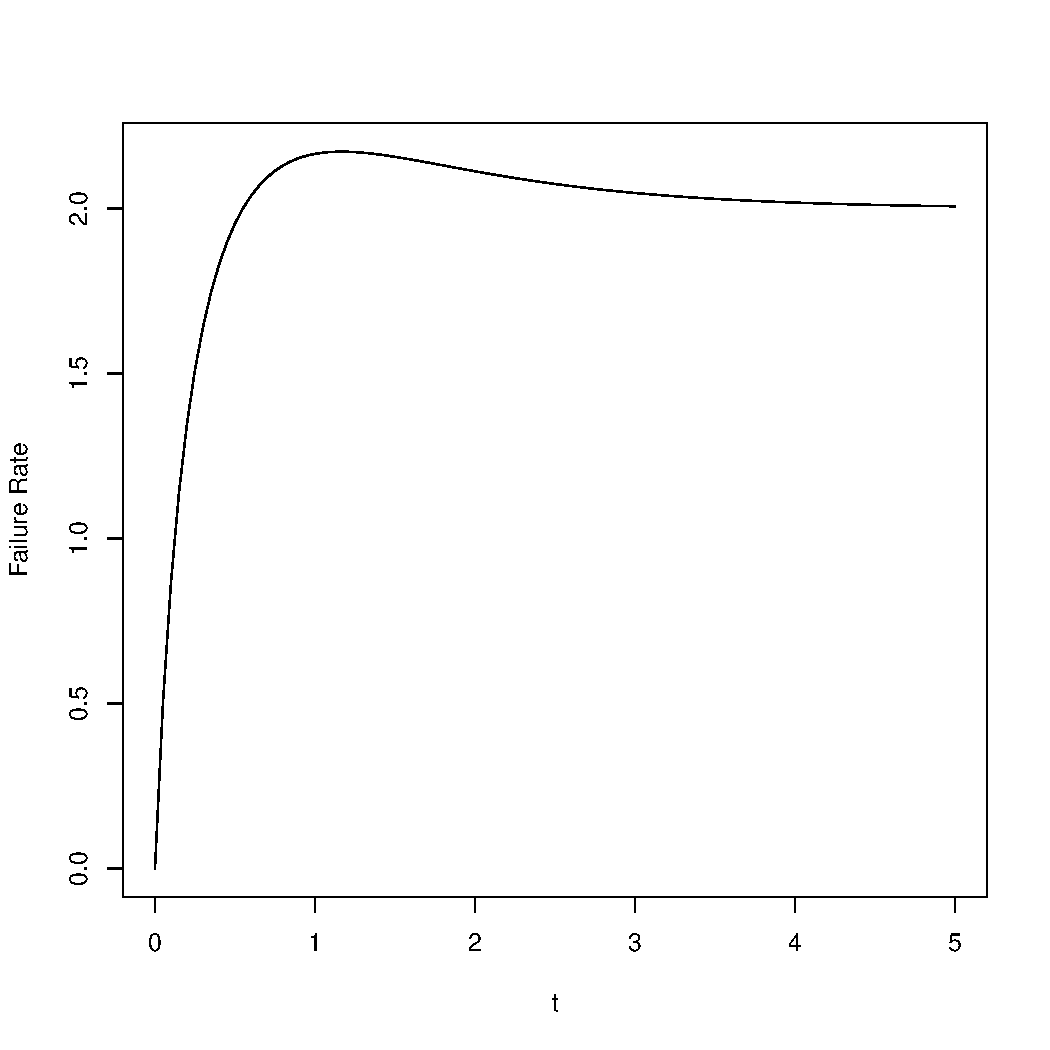
\includegraphics[width=0.5\linewidth]{art/hazard}
\caption{Failure rate of the parallel exponential component system.}
\label{fig:hazard_non_monotone}
\end{figure}





\begin{example}[Weibull Hazard]
The Weibull distribution is very common in reliability analysis since it is tractable generalization of the exponential distribution with many nice properties. 
It can be constructed by 
$\T := \lambda \U^{1/k}$, where $\U \sim \exp(1)$. 
This implies that for non negative $t$:
\begin{align}
	\pdf{\T}{t} &= \frac{k}{\lambda}\left(\frac{t}{\lambda} \right)^{k-1} e^{-(t/\lambda)^k}, \\
	\cdf{\T}{t} &= 1 - e^{-(t/\lambda)^k},
\end{align}
so that 
\begin{align}
	\survive{\T}{t} &= e^ {-(t/\lambda )^k}, \\
	\hazard{\T}{t} &= \frac{k}{\lambda} \left(\frac{t}{\lambda} \right)^{k-1} .
\end{align}
\end{example}
Elementary analysis shows that the hazard function of the Weibull may be increasing or decreasing in time ($\T$), depending on $k$, but it is always monotone.




\begin{example}[Gompertz Hazard]
	The Gompertz distribution\footnote{Not to be confused with it's generalization, the \emph{Gompertz-Makeham} distribution.} is another common distribution in reliability analysis. 
	\begin{align}
%	\pdf{\T}{t} &= \\
	\cdf{\T}{t} &= 1- e^\frac{-\lambda (\varphi^t-1)}{\log \varphi},
	\end{align}
	so that 
	\begin{align}
	\survive{\T}{t} &= e^\frac{-\lambda (\varphi^t-1)}{\log \varphi}, \\
	\hazard{\T}{t} &= \lambda \varphi^t .
	\end{align}
\end{example}
Elementary analysis shows that the hazard function of the Gompertz may be increasing or decreasing in time ($\T$), depending on $\varphi$, but it is always monotone.





\begin{example}[Empirical risk rates]
	\label{ex:bathtub}
When examining empirical risk rates of true devices, we almost always notice a \emph{bathtub} structure, such as in Figure~\ref{fig:bathtub}.\marginnote{Bathtub}
This shape captures the idea that products tend to fail more when they are brand new, or as they are very old, while their failure rates are fairly stable in the ``mid-life''.
In this text, we will not be providing a particular distribution which has this property. 
We refer the reader to \cite{nadarajah_bathtub-shaped_2008} for examples of distributions which have the bathtub property.
\end{example}


\begin{figure}[ht]
\centering
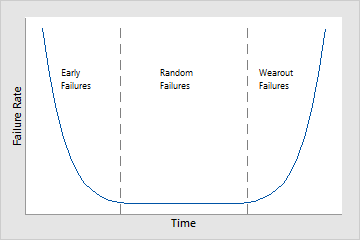
\includegraphics[width=0.5\linewidth]{art/bathtub_curve}
\caption[Bathtub empirical hazard curve]{Bathtub curve of empirical failure rates. \newline
\url{http://support.minitab.com/en-us/minitab/17/topic-library/modeling-statistics/reliability/distributions-in-reliability-analysis/hazard-functions/}}
\label{fig:bathtub}
\end{figure}




\subsubsection{Aging}
The idea of \emph{aging} is that failure rate may vary over time. It is an important concept in reliability, as demonstrated by the empirical bathtub failure rate (Figure~\ref{fig:bathtub}).
Instead of checking if a particular textbook distribution has some ageing property, we instead analyze classes of distributions with the desired notion of ageing.
Our goal will ultimately be to understand the ageing of a whole system, as a function of the ageing of its components.

\begin{definition}[IFR]
We call a failure time distribution to be in the \emph{increasing failure rate} (IFR) ageing class, if it has a non decreasing failure rate.
\end{definition}


\begin{definition}[IFRA]
We call a failure time distribution to be in the \emph{increasing failure rate average} (IFRA) ageing class, if the average risk is non decreasing in $t$. 
Formally: $\cuhazard{\T}{t}/t=\int_0^t \hazard{\T}{s}\dif s/t$ is non decreasing in $t$.
\end{definition}
The intuition underlying IFRA relies on understanding $\cuhazard{\T}{t}/t$, which can be seen as the average risk from ignition to time $t$. 
IFRA thus means that even if the risk decreases at some point in time, the average risk still increases. 


\begin{definition}[NBU]
We call a failure time distribution to be in the \emph{new better then used} (NBU) ageing class, if 
$\survive{\T}{t_1+t_2} \leq \survive{\T}{t_2} \survive{\T}{t_1}$.
\end{definition}


\begin{definition}[NBUE]
Define the \emph{expected residual life}, $\mu(t)$, to be 
$$\mu(t):= \expect{\T-t|\T>t}.$$
\marginnote{Expected Residual Life}
We call a failure time distribution to be in the \emph{new better then used in expectation} (NBUE) ageing class, if 
$\mu(t) \leq \mu(0)$.
\end{definition}
NBUE can be easily understood, since it means that a component's expected life is maximal when it is brand new. 


\begin{theorem}
$IFR \Rightarrow IFRA \Rightarrow NBU \Rightarrow NBUE. $
\end{theorem}


The following theorem states a relation between the ageing properties of particular components, and that of the whole system. In particular it states that for the (very wide) class of monotone systems, then the IFRA property is conserved. 
This should be contrasted with the IFR property, which is not conserved, as demonstrated by the parallel system in  Example~\ref{eg:failure_parallel}.
\begin{theorem}[IFRA closure theorem]
\label{thm:ifra_closure}
If the independent components of a monotone system are IFRA, then so is the whole system.
\end{theorem}


Series systems are a extremely small and particular subset of monotone systems.
It does provide, however, an example of systems where not only IFRA is preserved, but also the stronger IFR.
The following corollary follows immediately from Theorem~\ref{thm:ifr_closure} and the fact that a sum of monotone functions is monotone.
\begin{cor}[IFR closure for series systems]
\label{cor:ifr_series}
A series system of independent IFR components is IFR.
\end{cor}




Now consider a two-component system, where one component kicks-in when the first fails.
We will call this an \emph{offline backup}.\marginnote{Offline Backup}
The survival times of the components in an offline backup system are clearly dependent. 
It turns out that for such a system of IFR components, does conserve the IFR property, as seen in the following theorem.
\begin{theorem}[Convolution of IFR]
\label{thm:ifr_convolution}
For two independent random variables, $\x$ and $\y$, both in the IFR ageing class, then so is $\x+\y$.
\end{theorem}
The theorem is called the convolution theorem, because the distribution of a sum of independent random variables, is the convolution of their distributions.


\begin{extra}[IFR and log-concave]
The IFR requirement, is essentially the same as log-concavity of the density function.
This immediately implies many properties of the class, including the convolution theorem above.
See \cite{bagnoli_log-concave_2005}.
\end{extra}

\begin{example}[IFR of Gamma]
The Gamma (and thus the Erlang) distribution is in the IFR aging class, since it is the sum of exponentials, each IFR.
\end{example}

\begin{example}[Series system of offline backups]
What can we say about the ageing class of a series systems of offline backup systems? 
It turns out that if the components are IFR, then so will the whole system.
This is immediate from Corollary~\ref{cor:ifr_series} and Theorem~\ref{thm:ifr_convolution}.
\end{example}






\section{Statistical Analysis}
%TODO: update using Venables and Ripley (2002)

The probabilistic analysis of the previous section is great fun and all, but like any probabilistic problem, is has to be calibrated to real life. 
This is where data, and statistics come in.

The statistical analysis of time-to-event data is very important to many disciplines. 
It possibly started in the $17$'th century with the \emph{Life Tables} of John Graunt and
William Petty, used by actuaries to compute life expectancies. 
These were later reinvented and augmented to the full statistical framework known as \emph{failure-time} analysis in engineering, \emph{survival} analysis in epidemiology and biostatistics, and \emph{event-history} analysis in sociology. \marginnote{Failure-time analysis}

\begin{remark}[Reliability analysis versus failure-time analysis]
	In this text we use the term \emph{reliability analysis} for the probabilistic analysis above, and \emph{failure-time analysis} for the statistical problem. 
	We do so to respect the original literature where these originate. 
\end{remark}


The statistical analysis of failure data, is typically concerned with the estimation of the \textbf{hazard} function, or the \textbf{survival} function. 
To do so, we face the following statistical challenges:
\begin{description}
\item [Failure Distribution] like any statistical model, we will need to assume something about distributions of failure times.

\item [Identifiability] It is typically hard, if not impossible, to estimate the reliability of particular components, from the reliability of the whole system. 

\item [Censoring] A major concern with reliability data, is that in any finite length experiment, some events will just not have happened yet; their failure time will thus be \emph{censored}. Ironically- the more reliable a component, the less data we will have to estimate its reliability. 

\item [Lab versus real-life conditions] Reliable components take very long time to fail. We will thus extrapolate from harsh lab conditions to real-life operating conditions. This requires the introduction of covariates. 

\end{description}



\subsection{Failure distribution}
Assuming the distribution of the failure time is no different than the problem of assuming the sampling distribution in elementary statistical problems (e.g., in a t-test).
Luckily, there is one very popular estimator of the hazard function, which is \emph{non-parametric}, meaning that it is free of any distribution assumption.
\begin{definition}[Kaplan-Meier Estimator]
	The Kaplan-Meier estimator of the survival function $\survive{\T}{t}$ is defined as 
	\begin{align}
		\surviven{\T}{t}:=\prod_{t_i \leq t} \frac{n_i-d_i}{n_i},
	\end{align}
	where $t_i$ is the period between the $i-1$'th event and the $i$'th event, 
	$n_i$ is the number of units that did not fail until the end of $t_i$,
	$d_i$ is the number of units that fail in period $t_i$ (typically $1$, except for ties).
\end{definition}
The rational of the estimator is obvious once we realize that $\frac{n_i-d_i}{n_i}$ estimates the probability of \textbf{not} failing during period $t_i$, and that surviving all the way to time $t$ means not failing for all previous periods. 

Given a covariate, $x$, that splits into sub populations, one may estimate and compare the survival separately for each value of the covariate: $\surviven{\T|x}{t}$.






\subsection{Identifiability}

\begin{example}[Likelihood estimation of a series system]
\label{eg:likelihood_of_failures}
Assume a series system $\Phi$ with $p$ independent, exponential components with rates $(\lambda_1,\dots,\lambda_p)$.
We have $n$ observations on the failure times of the system $t_1,\dots,t_n$.
How can we estimate the failure rates?
To use a likelihood approach, we need the data's sampling distribution.
Denoting the failure time of the $j$'th component of the $i$th device with $\T_{i,j}$, we have that $\T_{i,j}\sim \exp(\lambda_j)$ by assumption.
Since the system is serial, then $\T_i=\min_j(\T_{i,1},\dots,\T_{i,p})$.
By the properties of the exponential distribution $\T_i \sim \exp(\lambda)$, where $\lambda:=\sum_{j=1}^{p} \lambda_j$, as we have already seen with the failure rate. It follows that
$\pdf{\T_i}{t}=\lambda \exp(-\lambda t)$.
We may then write the likelihood function, maximize it with respect to $\lambda$ and discover, as we already know, that $$\hat{\lambda}=\frac{n}{\sum_{i=1}^{n} t_i}.$$
We are now left with the problem of recovering $(\lambda_1,\dots,\lambda_p)$ from $\lambda$. 
Can we do it? On the face of it- no. Which should not surprise us, since the mere knowledge of a device failure, is not very informative on the particular component that failed, which we would need to estimate $(\lambda_1,\dots,\lambda_p)$.
\end{example}

Example~\ref{eg:likelihood_of_failures} teaches us that unless further assumptions are introduced, the estimation of the component-wise failure rates requires information on the component-wise failure times. 





\subsection{Censored Events}
Consider several components being analyze for their reliability. 
Ironically, we actually want them to fail. If they do not, they do not convey information on their reliability.
In the event that a component has not failed, we clearly cannot register its failure time. 
Omitting this component from the sample will upward bias the estimated reliability.
These events are called \emph{censored} observations. 

Decomposing the likelihood function, $\lik$, to the contributions of each independent event, $\lik=\prod_{i=1}^n \lik_i$, then the likelihood of non-censored events is given by
\begin{align}
	\lik_i=\density_\T(t_i)= \survive{\T}{t_i} \hazard{\T}{t_i},
\end{align}
and the likelihood of a censored event, under the \emph{non-informative} assumption, is given by 
\begin{align}
	\lik_i=\survive{\T}{t_i} .
\end{align}
Unifying the two cases assuming independent observations, using an indicator for non-censoring, $c_i$, and taking logs we have
\begin{align}
	\loglik &:=\log \lik\\ 
	&= \log \left[\prod_{i=1}^{n} \survive{\T}{t_i} \hazard{\T}{t_i}^{c_i}\right] \\
	&= \sum_{i=1}^{n} [c_i \log \hazard{\T}{t_i} - \cuhazard{\T}{t_i}]. \label{eq:censored_likelihood}
\end{align}


\begin{example}[Censored exponential lifetimes]
\label{ex:censoring}
Recalling that the failure rates of exponential lifetimes are fixed, we have that the likelihood of censored exponential lifetimes is given by 
$$
	\sum_{i=1}^{n} [c_i \log \lambda - \lambda t_i].
$$
The maximum likelihood estimator of $\lambda$ is thus
\begin{align}
	\estim{\lambda}= \frac{\sum c_i}{\sum t_i}. \label{eq:censored_ml}
\end{align}
Eq.(\ref{eq:censored_ml}) lends itself to a nice interpretation.
The numerator is the total number of failures.
The denominator is the total \emph{exposure time}. 
The estimated failure rate is thus the number of failures per unit of exposure time. 
\end{example}

The example also demonstrates that overly reliable components is a problem. 
If no component fails, i.e., all observations are censored, then $\sum c_i=0$, so that $\estim{\lambda}=0$. 
This is both mathematically true, and absolutely not interesting; we need events to occur for us to learn from them!
This motivates the use of covariates such as temperature, pressure, humidity, etc. to force failure events. 
The problem will then be how to convert failure rates in extreme conditions, to failure rates in regular conditions?
Sometime we have a physical theory that tells us what is the effects of various factors.
For instance, the \emph{Arrhenius model}, and the \emph{Eyring model} are physically motivated models that capture the effect of temperature.
For models for stress, voltage, humidity, and other life accelerating covariates, see for instance \cite[Sec.8.1.5]{natrella_nist/sematech_2010}
In the next section we introduce two very simple models to demonstrate how we deal with covariates. 



\begin{extra}
The results in Example~\ref{ex:censoring} is trivial if you consider failures as events which come as a Poisson process, which is implied from the exponential times assumption. 
The process is run for $\sum t_i$ time, and the total event count is $\sum c_i$. 
The trivial estimator for the rate of the process, is $\sum c_i/\sum t_i$.
\end{extra}






\subsection{From lab to reality: ``Accelerating Life''.}


\subsubsection{Accelerated Life model}
An \emph{accelerate life} model assumes that covariates rescale \emph{time}. 
For instance, the lab may produce conditions where time advances ten times faster than in real-life operating conditions.


The model is best understood as a \emph{log-linear} model, i.e., the effects of the various factors, $x$, are linear in log-of-time scale:
\begin{align}
\label{eq:estimating_accelerated_life}
	\log \T_i = x_i'\beta + \varepsilon_i,
\end{align}
for some error term $\varepsilon_i$. 

The definition of accelerated life models via Eq.(\ref{eq:estimating_accelerated_life}) is very convenient for practical purposes. 
It means that after taking the log of failure times, effects ($\beta$'s) can be estimated using any software that can solve a linear model. 

The accelerated life model, like any other log-linear model, implies that our factors have multiplicative effects.
To see this, compare the distribution of failure times at some condition $x_0$ versus some other condition $x_1$.
Taking the exponent of both sides of Eq.(\ref{eq:estimating_accelerated_life}) we have
\begin{align}
	\T_{x_1} = \T_{x_0} e^{\beta'(x_1-x_0)},
\end{align}
so we see that a change in the conditions from $x_0$ to $x_1$ multiplies failure times. 
This also explains why the models are called \emph{accelerated time}: this is because we can make time ``move'' multiplicatively faster or slower, by changing the operating conditions. 



\begin{think}
	Think of a single two-state factor, $x_i \in\set{0,1}$ to get some intuition to the meaning of the parameter $\beta$. 
\end{think}



\begin{example}[Accelerated life with Gaussian noise]
\label{eg:accelerated_gaussian}
The maximum likelihood estimation of $\beta$ when assuming that $\varepsilon_i \sim \gauss{0,\sigma^2}$, collapses to a simple linear regression when the dependent variable is simply $\log t_i$.
\end{example}


\begin{extra}[Tobit regression]
Assuming $\varepsilon_i \sim \gauss{0,\sigma^2}$, as in the previous example, implies that failure times are \emph{log normal} distributed. 
This approach is known as \emph{Tobit} regression.
\end{extra}







\subsubsection{Proportional Hazard Models}
The \emph{proportional hazard}, or \emph{proportional risk} class of models, assumes that covariates multiply not time, but rather failure rates. 
Put differently, accelerated rescales time linearly, thus hazards are rescaled non-linearly. Proportional hazards rescale hazards linearly, thus time is rescaled non-linearly. 
Qualitatively, they are the same. 
Quantitatively, the exact amount of acceleration (deceleration) may differ. 
The choice between these models typically depends on the underlying physical theory, and on the ease of computation and interpretation.


A proportional hazard model assumes that the risk function when operating under some conditions $x_0$ is related to the risk under conditions $x_1$ via:
\begin{align}
\label{eq:proportional_hazard}
	\hazard{\T|x_1}{t}:=\hazard{\T|x_0}{t} e^{\beta'(x_1-x_0)}  ,
\end{align}


\begin{think}
	Think of a single two-state factor, $x_i \in\set{0,1}$ to get some intuition to the meaning of the parameter $\beta$. 
\end{think}




The linear rescaling of the risk in the proportional hazard model, implies the following relation between survival functions
\begin{align}
\label{eq:survival_proportional_hazard}
	\survive{\T|x_1}{t}=\survive{\T|x_0}{t}^{\exp((x_1-x_0)'\beta)}.
\end{align}
To see this recall Eq.(\ref{eq:survival_to_hazard}):
\begin{align*}
\hazard{\T|x_1}{t} 
&=  - \frac{\partial}{\partial t} \log \survive{\T|x_1}{t}  \\
&= - \frac{\partial}{\partial t} \log \survive{\T|x_0}{t}^{\exp((x_1-x_0)'\beta)} \\
&= e^{(x_1-x_0)'\beta} - \frac{\partial}{\partial t}  \log \survive{\T|x_0}{t} \\
&=  \hazard{\T|x_0}{t} e^{(x_1-x_0)'\beta} 
\end{align*}
as required.






\begin{example}[Closure of the exponential failure times]
The exponential failure times have a nice property:
if the failure times are exponential under \textbf{some} condition, $x_0$, then they are exponential for \textbf{all} conditions. 
This holds if we assume that factors have an accelerated-time effect, or a proportional-hazard effect. 
Put differently: for the exponential distribution (only), a linear rescaling of time is equivalent to a linear rescaling of hazards. 
Put more differently: if we assume exponential failure times, the proportional-hazard model and the accelerated-life model are the same. \\
\textbf{Proof:}
The proportional-hazard case:
$\T_{x_0}\sim \exp(\lambda)$ by the exponential assumption, so that 
$\hazard{\T_{x_0}}{t}=\lambda$.
Now $\hazard{\T_{x_1}}{t}=\hazard{\T_{x_0}}{t} e^{\beta(x_1-x_0)}$ by the proportional hazard assumption, so that $\forall x_1: \hazard{\T_{x_1}}{t}= const$, which completes the proof that failure times are exponential under \textbf{all} conditions. \\
The accelerated-life case:
$\T_{x_0}\sim \exp(\lambda)$ by the exponential assumption, so that 
$e^{\varepsilon_i}$ is exponential.
Denoting $\gamma:=e^{\beta'(x_1-x_0)}$, then $\T_{x_1} = \gamma \T_{x_0} $ by the accelerated time assumption, so that $\forall x_1: \T_{x_1} \sim \exp(\lambda/\gamma)$, which completes the proof that failure times are exponential under \textbf{all} conditions. 
\end{example}








\subsection{Choosing the Base Failure Rate}
\label{sec:based-failure-rate}
In all the above models, we are free to choose the base failure rate: 
$\survive{\T_0}{t}$ in Eq.(\ref{eq:accelerated_life}), or
$\varepsilon$ in Eq.(\ref{eq:estimating_accelerated_life}), or 
$\hazard{\T|x_0}{t}$ in Eq.(\ref{eq:proportional_hazard}).
Three possible approaches include:
\begin{enumerate}
\item Assume a \textbf{parametric} model, such as exponential times, Weibull times, etc.
\item Assume a \textbf{semi-parametric} model, which can be simply seen as a flexible class of distributions, that has no particular parametric representation. In failure-time analysis, the \emph{piece-wise constant} hazard is a popular choice.
\item Do not assume anything on the distribution, known as a \textbf{non-parametric} approach. 
\end{enumerate}
If we assume a particular parametric model, then we may gather failure time data, write the likelihood function, and return failure rate estimates, and covariate effects.
We now focus on the more flexible framework of semi-parametric modelling.


\subsection{The Parametric Case}
A parametric model fitting to failure data, is simply a maximum likelihood problem.
Examples \ref{eg:likelihood_of_failures}, \ref{eg:accelerated_gaussian}, and \ref{eg:accelerated_exponential} demonstrate this. 



\subsection{The Semi Parametric Case}
We now relax the explicit failure time distribution assumption, and adopt a more flexible semi-parametric distribution class, known as the \emph{piecewise exponential class}.\marginnote{Piecewise Exponenitial}
Consider the proportional hazard model:
\begin{align}
	\hazard{\T|x_1}{t}:=\hazard{\T|x_0}{t} \times \exp((x_1-x_0)'\beta).
\end{align}
The model clearly requires some baseline failure rate $\hazard{\T|x_0}{t}$.
A flexible, yet not too flexible assumptions, is that the failure rate is constant in some time intervals:
\begin{align}
	\hazard{0}{t}=h_j \quad \text{if} \quad t\in [\tau_{j-1},\tau_j)
\end{align}
This class of distributions has $J(J-1)$ parameters: $(\tau_1,\dots,\tau_{J-1},h_1,\dots,h_J)$.
We are free to choose $J$. 
Large $J$ are very flexible classes, but will require a lot of failure data to estimate.
Small $J$ are less flexible, but require less data to estimate. 
At the limits, when $J=1$, we are back to exponential failure times. 
At the other limit, where $J \to \infty$, we have an absurdly flexible distribution class, which requires impossibly large amounts of data to estimate.

Since the failure rate is piece-wise constant, the distribution class is known as \emph{piece-wise exponential}.\marginnote{Piecewise Exponential}
It is a rather flexible class of distributions. Figure~\ref{fig:piecewise_exponential} depicts the approximation of the Weibull survival function, using a piece-wise constant hazard function, with $J=3$ and appropriate selected parameters.
\begin{figure}[ht]
\centering
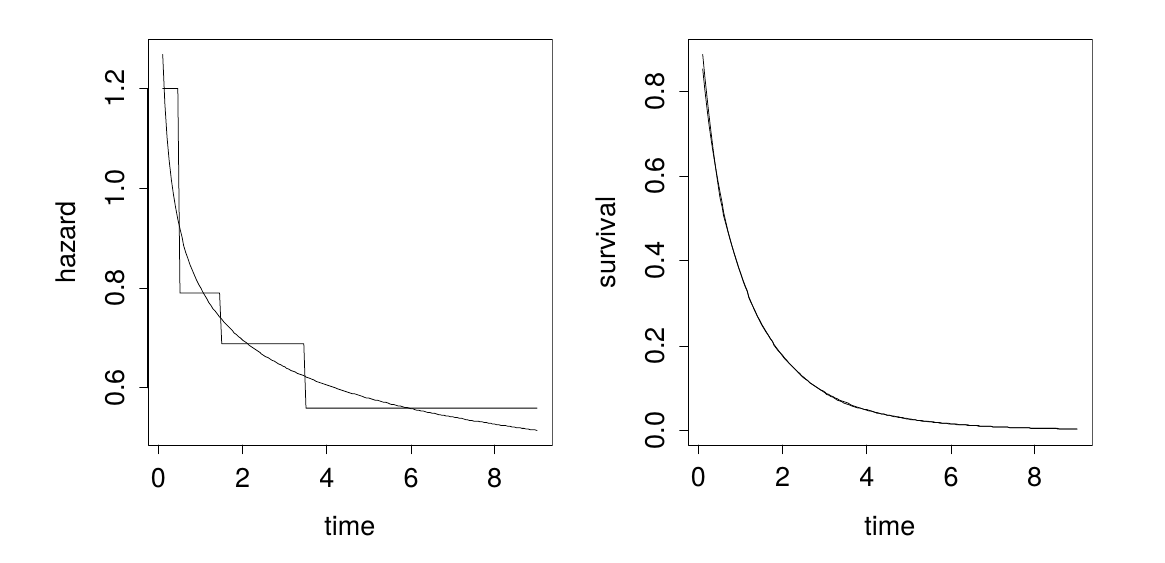
\includegraphics[height=0.2\textheight]{art/piecewise_exponential}
\caption{Piecewise Exponential aproximation of the Weibull distribution.}
\label{fig:piecewise_exponential}
\end{figure}


The piecewise-constant hazard model is very convenient to analyze under the proportional hazard assumption:
\begin{align}
	\hazard{x}{t} = \hazard{x_0}{t} e^{(x-x_0)'\beta} = h_j e^{(x-x_0)'\beta}.
\end{align}
There are $p+2J$ parameters to estimate.
This can be done directly using maximum likelihood, or by casting the problem as several separate Poisson regression problem. 
This has the benefit that the problem may be immediately solved with any statistical software suite, with existing numerical solvers.
We will currently not pursue this avenue, and refer the reader to the bibliographic notes.



\section{Collecting the pieces}
In this chapter we have seen the probabilistic reliability analysis, where we assumed components' reliabilities are known. 
We then proceeded to the statistical problem of estimating reliabilities from failure data.
We now glue collect these pieces to sketch a realistic analysis workflow, which would look roughly as follows:
\begin{enumerate}
\item Estimate reliability parameters by collecting component-wise failure data. Data is collected in a lab so that you may accelerate time and rescale to realistic operating conditions.
\item Perform the probabilistic analysis of the whole system using the estimated parameters.
\end{enumerate}


\begin{remark}[Interplay between probability and statistics]
There is obviously an interplay between the above stages:
In the statistical analysis, we want the least possible set of assumptions;
For the probabilistic analysis, the more we can assume, the more we can say about the system as a whole.
\end{remark}



\begin{remark}[What is a component?]
The notion of a ``system'' and a ``component'' is not well defined.
Indeed, for some purposes you may consider a system, as a component in a larger system.
For the statistical problem, a component is probably the smallest unit you can collect data on. At times, the smallest unit, may be the system as a whole.
\end{remark}




\section{Repairable systems}
In this section we return the a probabilistic analysis.
Unlike the previous sections, we now study systems which may be repaired after they fail.
We will thus want to study the state of the system at time $t$.
This state may depend on the number of failures and repairs performed on the system up to $t$.

We start with the introduction of some quantities of interest.
\begin{definition}[Point availability]
The point availability at time $t$, denoted $A(t)$ is defined as 
\begin{align}
	A(t):= \expect{\Phi_t}=P(\Phi_t=1) .
\end{align}
\end{definition}

\begin{definition}[Interval reliability]
When considering the availability in some time interval $J$, and denoting by $N_J$ the number of system failures in the interval, we may study
\begin{align}
	P(N_j\leq k) &\\
	M(J) &:= \expect{N_j} \\
	A(J) &:= P(\Phi_t=1), \forall t \in J.
\end{align}
\end{definition}


\begin{definition}[Interval downtime]
Denoting by $Y_J=\int_J (1-\Phi_t) dt$ the downtime during interval $J$, we may study
\begin{align}
	P(Y_j \leq y) &	\\
	A^D(J) := \frac{\expect{Y_J}}{|J|}
\end{align}
\end{definition}

\paragraph{Limiting measures} The particular time $t$, or interval $J$ are usually not of real importance in the sense that all times and intervals are equally important.
We will thus typically be interested in the above performance measures for in some \emph{steady state} of the systems, so that the measure is representative of all $t$ (or $J$), and thus no longer depends on $t$ (or $J$).
The typical approach for this is to study the limit of the performance measure, which implies the system has reached it's steady state. Formally, this means studying $\lim_{t \to \infty}$ of the above measures. 


We now start with the analysis of a \emph{single component} system, which we later complicate into \emph{multiple component systems}. 
The required theory is that of stochastic processes, in particular \emph{counting processes}. 
The reader is referred to the bibliographic notes for rigorous proofs and details. 

\subsection{Single component systems}
For a single component, $\Phi_t=\x(t)$. 
If the component fails, it is replaced or repaired. 
We denote by $T_k$ and $R_k$ and the (random) time of the $k$'th run, and repair, respectively.
We assume $T_k \sim F$ and $R_k \sim G$, independent.

\begin{definition}[MTTF]
We denote by $\mu_F=\expect{T_k}$, the \emph{mean time to failure} (MTTF).
\end{definition}


\begin{definition}[MTTR]
We denote by $\mu_G=\expect{R_k}$, the \emph{mean time to repair} (MTTR).
\end{definition}

Obviously, MTTR and MTTF are important characteristics of the single-component system.


\begin{theorem}[Stable point availability]
As $t \to \infty$
\begin{align}
	A(t) \to \frac{\mu_F}{\mu_F+\mu_G}.
\end{align}
\end{theorem}

\begin{theorem}[Stable failures per unit of time]

As $t \to \infty$, then with probability one
\begin{align}
	\frac{N_t}{t} \to \frac{1}{\mu_F+\mu_g}
\end{align}
\end{theorem}

\begin{theorem}[Stable unavailability]
As $t \to \infty$, then with probability one
\begin{align}
	A^D([0,t])=\frac{Y_t}{t} \to \frac{\mu_G}{\mu_F+\mu_G} 
\end{align}
	
\end{theorem}








\subsection{Multiple component systems}
We will now want to study the availability of a system of multiple repairable components.
The performance of the single-component system still apply, but the analysis now has to account for the fact that the state of the systems depends on the state of $n$ repairable components, assumingly independent.
By indexing the components with $i$, we denote $T_{i,k}, R_{i,k}$ for the uptime and repair time of the $k$'th failure of the $i$'th component. Their distributions are $F_i$ and $G_i$ respectively.
The system failures up to time $t$ is still $N(t)$, but not we also allow for component-wise processes $N_i(t)$, with expectations $M(t)$, and $M_i(t)$.

Denoting $A_i(t)$ the availability of component $i$ at time $t$, $A(t)$ the n-vector of reliabilities, and $A_\Phi(t)$ the whole system's reliability. 

[TODO:Complete from  \cite[Sec.4.3]{aven_stochastic_1999}]



\section{Bibliographic Notes}
An light introductory discussion, may be found in \cite{nahmias_production_2015}. 
The probabilistic analysis in this text is adapted from \cite{aven_stochastic_1999}.
The seminal reference probably being \cite{barlow_mathematical_1965}.
The statistical analysis is adapted from German Rodriguez's Generalized-Linear-Models class notes\footnote{\url{http://data.princeton.edu/wws509/notes/c7.pdf}.} and \cite[Ch.8]{natrella_nist/sematech_2010}.
For more on the statistical analysis, see Chapter 13 of the excellent \citet{venables_modern_2002} and references therein. 


% 